\section{Fredholm analysis of the integral representations}
\label{sec:analysis}
In this section, we establish how layer potential
representations of oscillatory Stokes velocity fields
can be used to compute Stokes eigenvalues.
%
The main results show that for certain representations
the resulting integral equation is not invertible precisely
when $k^2$ is an eigenvalue.
%
For the interior Dirichlet eigenvalue problem, this is
proved separately for a double layer representation on
simply connected domains in \cref{thm:dlmain} and
for a combined-field representation on multiply connected
domains in \cref{thm:cfmain}.
%

Before proving the main theorems, we require a number
of uniqueness results for oscillatory Stokes boundary
value problems.
%
To prove the uniqueness results, we follow the 
structure presented in Colton and Kress~\cite[Ch. 3]{colton1983integral}
for the scalar Helmholtz equation.
%
First, we define the interior boundary value problems
of interest, which is straightforward.
%
For the exterior problems, we introduce a radiation condition
for the equations and establish that, under certain assumptions,
the standard layer potentials satisfy the radiation condition.
%
By including the radiation condition, it is then
possible to define well-posed versions of the
exterior boundary value problems.
%
Then we derive a number of uniqueness
results for some standard boundary value problems
on exterior domains.


Along with the Fredholm alternative, these uniqueness
results are sufficient to prove
\cref{thm:dlmain,thm:cfmain}.
%
Once the main theorems are established,
the details of how to use the Fredholm determinant
as a numerical tool for computing the Stokes eigenvalues
follows in a straightforward manner from the results
in~\cite{zhao2015robust}.
%
We reproduce these results in the present
context for completeness.

\subsection{Boundary value problems --- interior}

Let $\Omega$ be a bounded domain with $C^2$ boundary
denoted by $\Gamma$.
The Dirichlet boundary problem specifies the
velocity of the fluid on the boundary, i.e.

\begin{definition}[Interior Dirichlet problem]
  Let $\ff \in C(\Omega)$ be given. Find $(\bu,p) \in A(\Omega)$
  such that
  \begin{equation}
  \begin{aligned} \label{eq:dir_interior}
    \Delta \bu + k^{2} \bu &= \nabla p \quad \bx \in \Omega \, ,\\
    \nabla \cdot \bu &= 0 \quad \bx \in \Omega \, ,  \\
    \bu &= \ff \quad \bx \in \Gamma \, .
  \end{aligned}
  \end{equation}
\end{definition}
Note that the divergence-free constraint for the oscillatory
Stokes equations implies a compatibility condition on the
Dirichlet data $\ff$, namely that
\begin{equation} \label{eq:dir_compat}
  \int_\Gamma \ff \cdot \bnu \, dS = 0 \; .
\end{equation}


Let $\bsigma$ denote the stress tensor associated with
field $(\bu,p)$. 
Specifying the surface traction, $\bt = \bsigma \cdot \bnu$,
on the boundary gives the Neumann boundary value
problem, i.e.

\begin{definition}[Interior Neumann problem]
  Let $\bg \in C(\Omega)$ be given. Find $(\bu,p) \in A(\Omega)$
  such that
  \begin{equation}
  \begin{aligned} \label{eq:neu_interior}
    \Delta \bu + k^{2} \bu &= \nabla p \quad \bx \in \Omega \, ,\\
    \nabla \cdot \bu &= 0 \quad \bx \in \Omega \, ,  \\
    \bt &= \bg \quad \bx \in \Gamma \, .
  \end{aligned}
  \end{equation}
\end{definition}

\subsection{A radiation condition for the oscillatory Stokes
  equation}

\begin{figure}
  \begin{center}
  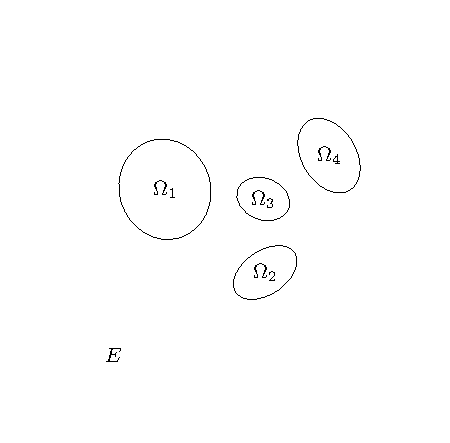
\includegraphics[width=0.4\textwidth]{media/ext_dom}
  \caption{Example of an exterior domain with four obstacles.}
  \label{fig:ext_dom}
  \end{center}
\end{figure}

Let $\Omega$ be the union of a finite collection of
simply connected domains, i.e. $\Omega = \bigcup_{i=1}^m \Omega_i$
for some $m \in \N$,
and let $E = \R^{2} \setminus \bar{\Omega}$ denote its
exterior; see \cref{fig:ext_dom} for an example with $m=4$.
%
Let $\Gamma = \partial E$ denote the boundary of $E$ and
$\bnu(\yy)$ denote the exterior normal to the point $\yy$ on
$\Gamma$, i.e. the normal vector pointing out of $E$ into $\Omega$.
%
For a given function $\ff$ defined on $\Gamma$,
the exterior Dirichlet boundary value problem is to
find a pair $(\bu,p)$ which satisfies:
\begin{equation}
\begin{aligned}
\Delta \bu + k^{2} \bu &= \nabla p \quad \bx \in E \, ,\\
\nabla \cdot \bu &= 0 \quad \bx \in E \, ,  \\
\bu &= \ff \quad \bx \in \Gamma \, . \nonumber
\end{aligned}
\end{equation}
In addition to the boundary condition on
$\Gamma$, we must impose radiation conditions
at $\infty$, analogous to the Helmholtz equation.
%

Let $B_r(0)$ denote the disc of radius $r$ centered
at the origin and $\partial B_r(0)$ its boundary.
%
We propose the following radiation condition.

\begin{definition} \label{def:radcond}
Let $(\bu,p)$ satisfy the oscillatory Stokes equations in
the exterior of a bounded domain. We say that
the pair $(\bu,p)$ is {\em radiating} if
\begin{equation}
\lim_{r\to \infty} \sqrt{r} \left| \bt - i k \bu \right| \to 0 \, ,
\label{eq:radcond}
\end{equation}
uniformly in direction where $\bt = \bsigma \cdot \bnu$
with $\bnu = \xx/|\xx|$, i.e. $\bt$ is the surface
traction on $\partial B_r(0)$.     
\end{definition}

\begin{thrm}
The oscillatory Stokeslet, as defined in \eqref{eq:ostokeslet}, 
satisfies the radiation condition in Definition \ref{def:radcond}.
Suppose that $\Gamma$ is the boundary of a region $\Omega$
and is $C^{2}$. 
Suppose that $\bmu \in C(\Gamma)$ and satsifies
$\int_{\Gamma} \bmu \cdot \bnu dS = 0$, where
$\bnu$ dentoes the outward normal to the curve $\Gamma$.
Then, the oscillatory Stokes 
double layer potential $\bD[\bmu]$, as defined in \eqref{eq:doublelayer},
also satisfies the radiation condition.
\end{thrm}

\begin{proof}
Consider the Stokeslet induced by an arbitrary charge
$k^2 \bpsi$ at the origin where $\psi \in \mathbb{C}^2$ 
is a constant. Let $r = |\xx|$,
$\bnu(\xx) = \xx/|\xx|$, and $\btau(\xx) = \bnu(\xx)^\perp$. We have

\begin{align*}
\bu (\xx) &= k^2 \GG(\xx,0) \bpsi \\
&= k^2 \left (-\II \Delta \Gbh(\xx,0)
+ \nabla \otimes \nabla \Gbh(\xx,0)\right ) \bpsi \\
&= -k^2 \left (\nabla^\perp \otimes \nabla^\perp \Gbh(\xx,0) \right) \bpsi \\
&= \left(\nabla^\perp \otimes \nabla^\perp \left ( \frac{1}{2\pi}
\log r + \frac{i}{4} H_0^{(1)} (kr) \right ) \right)\bpsi \; .
\end{align*}
Note that derivatives of $\log r$ are $\littleo (1/\sqrt{r})$
and that the pressure associated with the Stokeslet is
$p = \nabla \Glap(\xx) \cdot \bpsi$. We then have

\begin{align*}
\left | \sigma \cdot \bnu(\xx) - i k \bu \right | &=
\left | p \bnu(\xx) + \partial_{{\nu_x}} \bu + \nabla (\bu \cdot \bnu(\xx))
- ik \bu \right | \\
&\leq \left | \partial_{{\nu_x}} \bu - ik\bu \right | + \left | \nabla(\bu \cdot \bnu(\xx)) \right |
+ \littleo (1/\sqrt{r}) \\
&\leq \frac{1}{4} \left | \partial_{{\nu_x}} \left(\nabla^\perp \otimes
\nabla^\perp \left (H_0^{(1)} (kr) \right ) \right)\bpsi
- i k \left(\nabla^\perp \otimes \nabla^\perp
\left (H_0^{(1)} (kr) \right ) \right)\bpsi \right | \\
& \quad + \left | \nabla \left( \partial_{\tau_x} \left ( 
\nabla^\perp \left (H_0^{(1)} (kr) \right ) \cdot \bpsi  \right )
\right) \right | + \littleo (1/\sqrt{r}) \; .
\end{align*}
Because $H_0^{(1)}(kr)$ has the asymptotic expansion 

\begin{equation}
H_0^{(1)}(kr) = \sqrt{\frac{2}{\pi k r}} e^{i(rk-\pi/4)} \left ( 1 + O\left (
\frac{1}{r} \right ) \right ) \; \nonumber
\end{equation}
as $r\to \infty$, we have

\begin{equation}
\left | \partial_{{\nu_x}} \left(\nabla^\perp \otimes
\nabla^\perp \left (H_0^{(1)} (kr) \right ) \right)\bpsi
- ik \left(\nabla^\perp \otimes \nabla^\perp
\left (H_0^{(1)} (kr) \right ) \right)\bpsi \right | =
o ( 1/\sqrt{r} ) \; . \nonumber
\end{equation}
Finally, because $H_0^{(1)}(kr)$ is radially symmetric,
we have

\begin{equation}
\left | \nabla \left( \partial_{\tau_x} \left ( 
\nabla^\perp \left (H_0^{(1)} (kr) \right ) \cdot \bpsi  \right )
\right) \right | = 0 \; , \nonumber
\end{equation}
so that the Stokeslet satisfies the radiation condition.

For the double layer potential, we only establish the
decay of the pressure, which we will denote by $p^\bD$;
the rest of the terms in \eqref{eq:radcond} can be bounded
using an argument like that for the Stokeslet above.
Because $p^\bD$ is harmonic in the exterior of any disc
containing $\Gamma$, it is sufficient to show that
$|\nabla p^\bD| = \bigo (1/r^2)$. Let $\btau$ denote the
positively oriented tangent to the curve $\Gamma$ and
$\mu_\nu(\yy)$ and $\mu_\tau(\yy)$ denote $\bmu(\yy) \cdot \bnu(\yy)$ and
$\bmu(\yy) \cdot \btau(\yy)$, respectively. Substituting
$\bD \bmu$ into \eqref{eq:ostokes}, we obtain

\begin{align*}
\nabla p^\bD(\xx) &= (\Delta + k^2) \bD \bmu(\xx) \\
&= \int_\Gamma \left (-k^2 \nabla \Glap (\xx,\yy) +
2 \nabla^\perp \partial_{\nu\tau} \Glap (\xx,\yy) \right ) \mu_\nu(\yy)
\, dS(\yy) \\
& \qquad + \int_\Gamma \nabla^\perp (\partial_{\tau\tau}-\partial_{\nu\nu})\Glap \mu_\tau(\yy)
\, dS(\yy) \; .
\end{align*}
The other terms are higher-order derivatives
of $\Glap$, so it is sufficient to show that the term

\begin{align*}
|\nabla p_1(\xx)| &:= \left |-k^2 \nabla \int_\Gamma \Glap(\xx,\yy)
\mu_\nu(\yy) \, dS(\yy) \right |
\end{align*}
is $\bigo (1/r^2)$. In the following, let $z = x_1 + i x_2$ be the
point corresponding to $\xx$ in the complex plane and let $R$
be the radius of some disc containing $\Gamma$. If $|\xx| > 2R$,
we can use the standard multipole expansion of $\log(z-(y_1+iy_2))$
and the assumption that $\int_\Gamma \bmu \cdot \bnu = 0$
to obtain
\begin{align*}
|\nabla p_1(\xx)| &= \frac{k^2}{2\pi} \left |  \partial_z \int_\Gamma \log(z-(y_1+iy_2))
\mu_\nu(\yy) dS(\yy) \right | \\
&= \frac{k^2}{2\pi} \left |  \partial_z  \left ( \log(z) \int_\Gamma \mu_\nu(\yy) \, dS(\yy)
+ \sum_{l=1}^\infty \frac{1}{z^l} \int_\Gamma \left( y_1+iy_2 \right)^l \mu_\nu(\yy) \, dS(\yy)
\right ) \right | \\
&= \frac{k^2}{2\pi} \left | \sum_{l=1}^\infty \frac{-l}{z^{l+1}}
\int_\Gamma \left( y_1+iy_2 \right)^l \mu_\nu(\yy) \, dS(\yy) \right | \\
&= \bigo (1/r^2) \; .
\end{align*}
\end{proof}

\subsection{Boundary value problems --- exterior}

Let $E$ and $\Gamma$ be as in the previous subsection.
The radiation condition allows for a well-posed formulation
of the exterior boundary value problems, which we
summarize in
\cref{def:dir_exterior,def:neu_exterior} below.

\begin{definition}[Exterior Dirichlet problem]
  \label{def:dir_exterior}
  Let $\ff \in C(\Gamma)$ be given. Find $(\bu,p) \in A(E)$
  such that
  \begin{equation}
  \begin{aligned} \label{eq:dir_exterior}
    \Delta \bu + k^{2} \bu &= \nabla p \quad \bx \in E \, ,\\
    \nabla \cdot \bu &= 0 \quad \bx \in E \, ,  \\
    \bu &= \ff \quad \bx \in \Gamma \, , 
  \end{aligned}
  \end{equation}
  and $(\bu,p)$ satisfies the radiation condition in
  \cref{def:radcond}.
\end{definition}
\begin{definition}[Exterior Neumann problem]
  \label{def:neu_exterior}  
  Let $\bg \in C(\Gamma)$ be given. Find $(\bu,p) \in A(E)$
  such that
  \begin{equation}
  \begin{aligned} \label{eq:neu_exterior}
    \Delta \bu + k^{2} \bu &= \nabla p \quad \bx \in E \, ,\\
    \nabla \cdot \bu &= 0 \quad \bx \in E \, ,  \\
    \bt &= \bg \quad \bx \in \Gamma \, ,
  \end{aligned}
  \end{equation}
  and $(\bu,p)$ satisfies the radiation condition in
  \cref{def:radcond}.
\end{definition}



\subsection{Uniqueness results}

Before moving on to the exterior uniqueness theorems,
we establish the well-known result that
the $k$ corresponding to interior eigenvalues, $k^2$,
are real-valued.

\begin{thrm}
  Let $\Omega$ be a bounded domain and suppose that
  $\Im (k) \neq 0$. Then both the interior
  Dirichlet and Neumann boundary value problems have
  unique solutions.
\end{thrm}
\begin{proof}
  A couple applications of the divergence theorem establish
  that
  \begin{equation} \label{eq:greenlike}
    \int_\Omega |2\be(\bu)|^2 - \overline{k}^2 |\bu|^2 \, dV
    = \int_\Gamma \bu \cdot \overline{\bt} \, dS \; . 
  \end{equation}
  Suppose that either $\bu = 0$ or $\bt = 0$ on $\Gamma$.
  Then, the right hand side of \cref{eq:greenlike} is
  zero. 
  Taking the real and imaginary parts of \cref{eq:greenlike},
  it is clear that $\bu \equiv 0$, if $\text{Im}(k) \neq 0$.
\end{proof}

The following lemmas are useful in establishing the uniqueness
of oscillatory Stokes boundary value problems.

\begin{lem}
  \label{lem:rep}
  Let the unbounded region $E$ be given as the exterior
  of a finite collection of bounded domains.
  Suppose that $(\bu,p)$ satisfies the oscillatory Stokes equation in 
  $E$ as well as the radiation condition~\cref{eq:radcond}. 
  Then 
  \begin{multline}
    \label{eq:repinfest}  
    \lim_{r\to\infty}
    \int_{|\by|=r} \left( |\bt|^2 + |k|^2 |\bu|^2 \right) dS +
    2 \Im(k) \int_{E \cap B_{r}(0)} \left(|k|^2 |\bu|^2 + |2\be(\bu)|^2 \right)
    dV \\
    = 2 \Im \left( k \int_{\Gamma} \bu \cdot
\overline{\bt} dS  \right) 
  \end{multline}
  
\end{lem}

\begin{proof}
Since $(\bu,p)$ satisfies the radiation condition, we have that
\begin{equation}
\lim_{r\to\infty} \int_{|\by|=r} | \bt - i k \bu|^2 dS = 
\lim_{r\to\infty} \int_{|\by| =r} \left( |\bt|^2 + |k|^2|\bu|^2 + 2 \Im 
\left( k \bu\cdot \overline{\bt} \right) dS \label{eq:raddecayproof1}
\right) = 0 \, . 
\end{equation}
Since $\bu$ satisfies the oscillatory Stokes equation $E \cap B_{r}(0)$,
using a couple of applications of the divergence theorem, we have that
\begin{equation}
\int_{E\cap B_{r}(0)} |2 \be(\bu)|^2 dV =
\int_{\Gamma} \bu \cdot \overline{\bt} dS
+ \int_{|\by|=r} \bu \cdot \overline{\bt} dS + \overline{k}^2 
\int_{E \cap B_{r}(0)} |\bu|^2 dV \,. \label{eq:raddecayproof2}
\end{equation}
Combining~\cref{eq:raddecayproof1,eq:raddecayproof2}, we get
\begin{multline*}
\lim_{r\to\infty} \int_{|\by|=r}\left(|\bt|^2 + |k|^2 |\bu|^2 \right) dS 
+ 2 \Im(k)\int_{E \cap B_{r}(0)} \left(|2\be(\bu)|^2 + |k|^2 |\bu|^2 
\right) dV \\
= 2\Im \left ( k \int_{\Gamma} \bu \cdot \overline{\bt} dS \right) \, .
\end{multline*}
\end{proof}

In the next lemma, we prove the analogue of Rellich's lemma for the
oscillatory Stokes equation. 
\begin{lem}
  \label{lem:rellich}
  Let the unbounded region $E$ be given as the exterior
  of a finite collection of bounded domains.
  Suppose $k$ is real, $\bu$ satisfies the oscillatory
  Stokes equation in $E$, and that 
\begin{equation}
\lim_{r \to \infty} \int_{|\by|=r} |\bu|^2 dS = 0 
\, . \label{eq:decayatinf}
\end{equation}
Then each component of $\bu$ is harmonic in $E$.
\end{lem}
\begin{proof}
We first note that each component of $\bu= (u_{1},u_{2})$ satisfies the 
oscillatory biharmonic equation in $E$, i.e.
\begin{equation}
\Delta (\Delta + k^2) u_{j} = 0 \quad j=1,2 \,. \nonumber
\end{equation}
For $r$ sufficiently large, we can express $u_{j}$ in the Fourier basis as
\begin{equation}
u_{j}(r,\theta) = \sum_{n=-\infty}^{\infty} a_{j,n}(r) e^{i n \theta}  \quad 
j=1,2 \, . \nonumber
\end{equation}
Using Parseval's identity then
\begin{equation}
\int_{|\by|=r} |\bu|^2 dS = r\sum_{n=-\infty}^{\infty} |a_{1,n}(r)|^2  +
|a_{2,n}(r)|^2 \, . \nonumber
\end{equation}
Since $\bu$ satisfies~\cref{eq:decayatinf}, we conclude that
\begin{equation}
\lim_{r\to\infty} r|a_{j,n}(r)|^2 = 0 \quad j=1,2 \, , \label{eq:adecay}
\end{equation}
Since $u_{j}$, $j=1,2$ satisfies the oscillatory biharmonic equation,
the functions $a_{j,n}$ are linear combinations of 
\begin{equation}
r^{|n|}, r^{-|n|}, H^{(1)}_{n}(k r), H^{(2)}_{n}(k r) \, , \quad
n\neq 0 \, , \nonumber
\end{equation}
and
\begin{equation}
1, \log{(r)}, H^{(1)}_{0}(k r), H^{(2)}_{0}(k r) \quad n=0 \, ,  \nonumber
\end{equation} 
where $H_{n}^{(1),(2)}(\cdot)$ are the Hankel functions of the first and
second kind of order $n$.
Since $a_{j,n}(r)$ satisfy~\cref{eq:adecay}, and using the asymptotic 
expansion of $H_{n}^{(1),(2)}(kr)$ when $k$ and $r$ are real-valued, we note
that the projection of $a_{j,n}$ on $r^{|n|}$, and $H_{n}^{1,2}(k r)$
must be zero. Thus, 
\begin{equation}
u_{j}(r,\theta) = \sum_{n=-\infty}^{\infty} \frac{a_{j,n} e^{i n \theta}}{r^{|n|}} 
\, , \nonumber
\end{equation}
for sufficiently large $r$.
Finally, by \cref{cor:analytic}, $\bu$ is
analytic in $E$. Therefore, each $u_j$ is harmonic
throughout $E$.
\end{proof}

\begin{remark} \label{rmk:harmu}
  Note that if $\bu$ satisfies the assumptions
  of~\cref{lem:rellich}, then each component is harmonic
  and thus $\bu$ satisfies
\begin{align}
k^2 \bu &= \nabla p \label{eq:massconsred} \; .
\end{align}
\end{remark}

\begin{remark}
  It should be noted that in~\cref{lem:rellich}, $\bu$ need
  not be a radiating solution. All that is assumed of $\bu$
  is that it satifies the PDE in $E$.
\end{remark}

We now have the results needed to establish the
uniqueness of exterior boundary value problems.

\begin{thrm}[Uniqueness of the Exterior Dirichlet Problem]
  \label{thrm:unique_dir_ext}
  Let the unbounded region $E$ be given as the exterior
  of a finite collection of bounded domains.
  Suppose that $\Im(k)\geq 0$ and 
  that $(\bu,p)$ is a radiating solution to the oscillatory Stokes
  equation in $E$ with $\bu =0$ on the boundary $\Gamma$, then
  $\bu \equiv 0$ in $E$.
\end{thrm}

\begin{proof}
Since $\bu = 0$ on $\Gamma$, it follows from~\cref{lem:rep} that
\begin{equation}
\lim_{r\to\infty}
\int_{|\by|=r} \left( |\bt|^2 + |k|^2 |\bu|^2 \right) dS +
2 \Im(k) \int_{E \cap B_{r}(0)} \left(|k|^2 |\bu|^2 + |\be(\bu)|^2 \right)
dV = 0 \nonumber
\end{equation}

Suppose that $\Im(k) > 0$. Then, it is immediate that
$\bu \equiv 0$ in $E$.

Suppose that $k$ is real valued. It is clear that
\begin{equation}
\lim_{r\to\infty} \int_{|\by|=r} |\bu|^2 dS = 0 \, . \nonumber
\end{equation}
Thus, the conditions on $\bu$ and $k$ in~\cref{lem:rellich}
are satisfied, and each component of $\bu$ is a harmonic function
with $\bu \to 0$ as $r \to \infty$. Furthermore, since $\bu=0$ on
$\Gamma$, by the uniqueness of solutions to the
Dirichlet problem for Laplace's equation
on exterior domains, we conclude that $\bu \equiv 0$
in $E$.
\end{proof}

\begin{thrm}[Uniqueness of the Exterior Neumann Problem]
  Let the unbounded region $E$ be given as the exterior
  of one simply connected domain.
  Suppose that $\Im(k)\geq 0$ and 
  that $(\bu,p)$ is a radiating solution to the oscillatory Stokes
  equation in $E$ with $\bt = 0$ on the boundary $\Gamma$, then
  $\bu \equiv 0$ in $E$.
\end{thrm}

\note{Manas: check out new argument below.}

\begin{proof}
Since $\bt = 0$ on $\Gamma$, it follows
from~\cref{eq:repinfest} that
\begin{equation}
\lim_{r\to\infty}
\int_{|\by|=r} \left( |\bt|^2 + |k|^2 |\bu|^2 \right) dS +
2 \Im(k) \int_{E \cap B_{r}(0)} \left(|k|^2 |\bu|^2 + |\be(\bu)|^2 \right)
dV = 0 \; . \nonumber
\end{equation}

Suppose that $\Im(k) > 0$. It is then immediate
that $\bu \equiv 0$ in $E$.

Suppose that $k$ is real. It is clear that
\begin{equation}
\lim_{r\to\infty} \int_{|\by|=r} |\bu|^2 dS = 0 \, . \nonumber
\end{equation}
Thus, the conditions on $\bu$ and $k$ in \cref{lem:rellich}
are satisfied, and each component of $\bu$ is a harmonic function
with $\bu \to 0$ as $r \to \infty$. Furthermore, as observed
in \cref{rmk:harmu}, $k^2 \bu = \nabla p$. Then, the boundary
condition becomes $0 = \bt = -p \bnu + 2 \nabla \partial_\nu p/k^2$.
Because $0 = \btau \cdot \bt = 2\partial_{\tau\nu} p/k^2$,
$\partial_\nu p $ is a constant on $\Gamma$.
Observe that $|\bu|$ and $|\be(\bu)|$ must be $O(1/r)$ as
$r\to\infty$. Thus,
for a radiating pair $(\bu,p)$ with $p$ harmonic,
we have that $|p| = O(1/r)$ and $|\nabla p| = O(1/r^2)$
as $r\to\infty$.
Using this bound and that $p$ is harmonic,
the divergence theorem implies that $\partial_\nu p=0$ on $\Gamma$.
Thus, $\bt = -p\bnu$ so that $p = 0$ on $\Gamma$. By the uniqueness
of solutions to the Dirichlet problem for Laplace's equation,
we have that $p=0$ so that $\uu \equiv 0$.
\end{proof}

\begin{remark}
For proving the correspondence between Stokes eigenvalues
for bounded regions, $\Omega$, and the non-invertibility
of corresponding second kind integral equations defined on
the boundary, $\Gamma$, we only need the uniqueness result
for the Neumann problem in the exterior of a single
simply connected domain. The proof of the exterior
Neumann problem in the exterior of several
obstacles is more involved and presented
in~\cref{app:neuuniqueness}.
\end{remark}

\begin{thrm}[Uniqueness of the Exterior Impedance Problem]
  Let the unbounded region $E$ be given as the exterior
  of a finite collection of bounded domains.
  Suppose that the complex numbers $\eta$ and $k$ satisfy that
  $\Re(\eta), \Re(k) > 0$ and $\Im(\eta),\Im(k) \geq 0$.
  Suppose further that
  $(\bu,p)$ is a radiating solution of the
  oscillatory Stokes equation in $E$ which satisfies
  the homogeneous impedance boundary condition
  \begin{equation}
\bt - i \eta \bu = 0 \quad \xx \in \Gamma \, . \nonumber
\end{equation}
Then $\bu \equiv 0$ for $\xx \in E$.
\end{thrm}

\begin{proof}
Since $\bu$ satisfies the radiation condition at $\infty$ and $\bt = i\eta \bu$
on $\Gamma$, it follows from~\cref{eq:repinfest} that
\begin{align*}
0 &=
\int_{|\by|=r} \left( |\bt|^2 + |k|^2 |\bu|^2 \right) dS +
2 \text{Im}(k) \int_{E \cap B_{r}(0)} \left(|k|^2 |\bu|^2 + |2\be(\bu)|^2 \right)
dV \nonumber \\
& \qquad - 2 \text{Im} \left( k \int_{\Gamma} \bu \cdot \overline{\bt} dS  \right) \\
&= 
\int_{|\by|=r} \left( |\bt|^2 + |k|^2 |\bu|^2 \right) dS +
2 \text{Im}(k) \int_{E \cap B_{r}(0)} \left(|k|^2 |\bu|^2 + |2\be(\bu)|^2 \right)
dV \nonumber \\
& \qquad + 2 \left( \left (\Re(k)\Re(\eta) + \Re(k)\Re(\eta)
\right ) \int_{\Gamma} |\bu|^{2} dS  \right)
\, .
\end{align*}
Because all of the quantities in the last expression above are
nonnegative, we have that
\begin{equation}
  \int_{\Gamma} |\bu|^{2} = 0 \implies \bu = 0  \quad \xx \in \Gamma \, .
  \nonumber
\end{equation}
The result then follows from the uniqueness of solutions to the exterior
Dirichlet problem.
\end{proof}

\subsection{The integral equations and their null-spaces}

\begin{figure}
\begin{center}
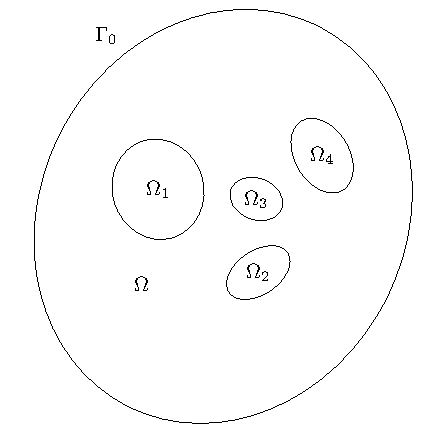
\includegraphics[width=0.4\textwidth]{media/mc_dom}
\end{center}
\caption{Example of a multiply connected domain with four obstacles.}
\label{fig:mc_dom}
\end{figure}

In this section, we establish the correspondence between
Stokes eigenvalues and the invertibility of certain integral
equations arising from layer potential representations
of solutions to the oscillatory Stokes equation.

Let $\Omega$ be a bounded domain given as
the intersection of a simply connected domain $\Omega_0$ and
the exteriors of a finite collection of bounded,
simply connected domains $\{ \Omega_i \}_{i=1}^m$
whose closures are contained in $\Omega_0$;
see \cref{fig:mc_dom} for an example with four inclusions.
Note that the
exterior of $\Omega$, which we denote by $E$, is the
disjoint union of the exterior of $\Omega_0$, which we
denote $E_0$, with the sets $\{ \Omega_i \}_{i=1}^m$.
Let $\Gamma$ denote the boundary of $\Omega$ with the normal
$\bnu$ pointing out of $\Omega$.
We will use superscript $+$ and $-$ signs
to indicate the limit values of a function on $\Gamma$
as approached from the exterior and interior, respectively.

For the sake of brevity, we consider only the
Dirichlet eigenvalue problem but a similar analysis
could be applied to the Neumann eigenvale problem.
We analyze two different representations for the
Dirichlet problem: a double layer potential,
i.e. setting $\bu=\bD_{k} \bmu$, and a combined-field
layer potential, i.e. setting
$\bu=(i\eta \bS_{k} + \bD_{k})\bmu$. 
While both representations result in a second kind
integral equation for the oscillatory Stokes Dirichlet
problem, the double layer potential has spurious non-trivial
nullspaces on domains with positive genus, as
explained below.

\begin{remark}
  The application of the Fredholm alternative here
  again follows the structure used for the Laplace
  eigenvalue problem in~\cite[Ch. 3]{colton1983integral}.
\end{remark}


\subsubsection{Dirichlet eigenvalues --- double layer
  representation}
\label{subsec:dlanalysis}
Suppose that the solution to the oscillatory
Stokes Dirichlet problem, \cref{eq:dir_interior},
is represented using a double layer potential defined
on $\Gamma$, i.e. setting $\bu = \bD_{k} \bmu$ for
an unknown density $\bmu$. 
Substituting this expression
into the boundary condition and applying
\cref{lem:jump-conds}, we obtain

\begin{equation}
  (\cI - 2\cD_{k}) \bmu = -2\ff \; . \label{eq:inteq_dir_int}
\end{equation}

The rank deficiency of $\cI-2\cDk$ is
well-known~\cite{biros2002embedded} and we summarize it
in

\begin{lem}[\cite{biros2002embedded}]
  \label{lem:nunull} In the notation above,
  $\bnu \in \cN(\cI - 2\cDkt)$.
\end{lem}
\begin{proof}
From~\cref{lem:propnullspacecorr}, we note that
$W[(\cI - 2\cD_{k})\bmu] =0$ implies that
$\left<(\cI -2\cD_{k})\bmu ,\bnu \right> = 0$ for
all $\bmu$, i.e. $\bnu \in R(\cI - 2\cD_{k})^{\perp}$, where
$R(A)$ denotes the range of the operator $A$. 
By the Fredholm alternative, the result then follows.
\end{proof}
Thus, we instead analyze the equation
\begin{equation}
(\cI - 2\cD_{k}  -2\cW) \bmu = -2\ff \; \, . \label{eq:inteq_dir_int_mod}
\end{equation}
Note that if $\ff$ satisfies the compatibility
condition $\int_\Gamma \ff \cdot \bnu \, dS =0$, then
\cref{eq:inteq_dir_int_mod} implies \cref{eq:inteq_dir_int}.

On simply connected domains, there is a one-to-one correspondance between
the eigenvalues of the Dirichlet problem for
the Stokes equation
and the values of $k$ for which the operator $(\cI - 2\cD_{k} - 2\cW)$
is not invertible. To prove this, we require the results
above and the following lemma:
\begin{lem}
  \label{lem:nutracli}
  If $\bt^{-}$ is the surface traction associated
  with an interior Dirichlet Stokes eigenfunction $\bu$,
  then $\bt^{-}$ and $\bnu$ are linearly independent.
\end{lem}
\begin{proof}
We first note that $\bS_{k}[\bnu](\bx) = 0$ for all $\bx \in \Omega$.
This follows from the application of the divergence theorem and the fact that
oscillatory Stokeslet is divergence free in $\Omega$. 
If $\bt^{-}$ is a surface traction associated with a Stokes eigenvalue, then
using Green's theorem, it follows that
$\bS_{k}[\bt^{-}](\bx) = \bu(\bx) \neq 0$ for $\bx \in \Omega$ and
thus $\bt^{-}$ and $\bnu$ are linearly independent.
\end{proof}

We now have

\begin{thrm}
\label{thm:dlmain}
Suppose that $\Omega$ is a bounded, simply connected domain. Then, the operator
$(\cI - 2\cD_{k} - 2 \cW)$ is not invertible if and only if $k^2$ is a
Dirichlet eigenvalue for the Stokes equation on $\Omega$.
\end{thrm}
\begin{proof}
  Suppose that $k^2$ is not a Dirichlet eigenvalue for
  the Stokes equation on
$\Omega$. 
Suppose further that $\bmu$ satisfies
\begin{equation}
(\cI - 2\cD_{k} - 2\cW) \bmu = 0 \, , \label{eq:dlproofrep}
\end{equation}
i.e. $\bmu$ is in the null-space
of $(\cI - 2 \cD_{k} - 2 \cW)$. 
Applying the operator $\cW$ to~\cref{eq:dlproofrep} and 
using~\cref{lem:propnullspacecorr}, we get
\begin{equation}
0 = \cW [(\cI - 2\cD_{k} - 2\cW)\bmu] = -2\cW [\bmu] \, .
\end{equation}
Thus~\cref{eq:dlproofrep} reduces to
\begin{equation}
(\cI - 2 \cD_{k})\bmu = 0\, .
\end{equation}
Suppose now $\bu = -2\bD_{k}[\bmu]$ in $\Omega$.
Then $\bu$ is a solution to the oscillatory Stokes equation in $\Omega$,
and applying~\cref{lem:jump-conds}, we get that the interior
limit of the velocity $\bu^{-}$, is given by $(\cI - 2\cD_{k}) \bmu = 0$
on $\Gamma$. Since $k^2$ is not a Dirichlet eigenvalue for the Stokes
equation on $\Omega$, we conclude that $\bu \equiv 0$ in $\Omega$. 
In particular, this implies that the interior limit of the surface traction
denoted by $\bt^{-} = 0$ on $\Gamma$. 
Using~\cref{lem:jump-conds} again, we conclude that the exterior limit
of the surface traction, $\bt^{+}$, is $0$ on $\Gamma$. 
Note that $\bu$ is a radiating solution of the oscillatory
Stokes equation in the exterior $E$, as $\cW[\mu] = 0$ implies
$\int_{\Gamma} \bmu \cdot \bnu = 0$.
From the uniqueness of the Neumann problem in the
exterior $E$, we conclude that $\bu \equiv 0$ in $E$ as well,
which in particular implies that
the exterior limit of the velocity, $\bu^{+}$, is $0$ on $\Gamma$.   
Using the jump conditions in~\cref{lem:jump-conds} again, we
get that $\bmu = \frac{1}{2}(\bu^{+} - \bu^{-}) = 0$.
Thus $(\cI - 2\cD_{k} - 2\cW)$ is invertible if $k^2$
is not a Dirichlet eigenvalue for the Stokes equation on $\Omega$.

From \cref{thrm:rep-theorem} we have 
  \begin{equation} 
    \bS_{k} [\bt](\xx) - \bD_{k}[\bu](\xx) = \begin{cases} 
    \bu(\xx) &\quad \xx \in \Omega \, , \\
    0 &\quad \xx \in E \; .
    \end{cases}
  \end{equation}
  Suppose that $k^2$ is a Dirichlet eigenvalue for the Stokes equation
  on $\Omega$ and let $\bu$ denote the corresponding eigenfunction
  with $\bt^{-}$ the corresponding surface traction on the
  boundary $\Gamma$.
  Since $\bu$ is a Dirichlet eigenfunction, the velocity restricted
  to the boundary, $\bu^{-}$, is $0$. 
  Using the Green's theorem representation for the pair
  $(\bu,\bt^{-})$ and evaluating the surface traction
  using~\cref{lem:jump-conds}, we get
  \begin{equation}
    \bt^{-} = (\cDt_{k} + \frac{1}{2} \cI) \bt^{-} \,
    \implies \left(\cI - 2\cDt_{k} \right) 
    \bt^{-} = 0 \, .
  \end{equation}
  From the above and \cref{lem:nunull,lem:nutracli},
  we know that $\bt^{-}, \bnu \in \cN(\cI - 2\cDt_{k})$
  are two linearly independent vectors in the null space.
  Let $c = \left< \bt^{-},\bnu \right>$. Then, it
  follows that $\left<\bt^{-} -c \bnu, \bnu \right> = 0$
  and thus $\cW[\bt^{-} - c\bnu] = 0$. 
  Since $\bt^{-}$ and $\bnu$ are linearly independent, we note that
  $\bt^{-} -c\bnu \neq 0$. Combining these results, we get that
  $(\cI - 2\cDt_{k} - 2\cW) (\bt^{-} - c\bnu) = 0$. 
  Since $\bt^{-}-c\bnu$ is non-trivial, and $\cW$ is
  self-adjoint, it follows from the Fredholm alternative
  that the operator $\cI - 2\cD_{k} - 2\cW$ is also not
  invertible.
\end{proof}

The correspondence result above does not hold on multiply
connected domains.
In particular, while the operator $\cI -2\cD_{k} -2\cW$ 
is indeed not invertible when $k^2$ is a Dirichlet eigenvalue,
it turns out that the operator is also not
invertible when $k^2$ is a Neumann eigenvalue
corresponding to the interior of one of the obstacle regions,
i.e. one of the $\Omega_{i}$ with $i > 0$. The following theorem
proves this result for a region with one obstacle;
the extension to the general case is straightforward.

\begin{thrm}
  Suppose that $\Omega$ is a multiply connected domain
  given by the intersection of a domain $\Omega_{0}$
  and the exterior of a single domain $\Omega_{1}$ with
  $ \bar\Omega_1 \subset \Omega_0$.
  Then, the operator $\cI - 2\cD_{k} - 2\cW$ has a non-trivial
  null space if $k^2$ is a Neumann eigenvalue of $\Omega_{1}$.
\end{thrm}

%\begin{figure}
%\begin{center}
%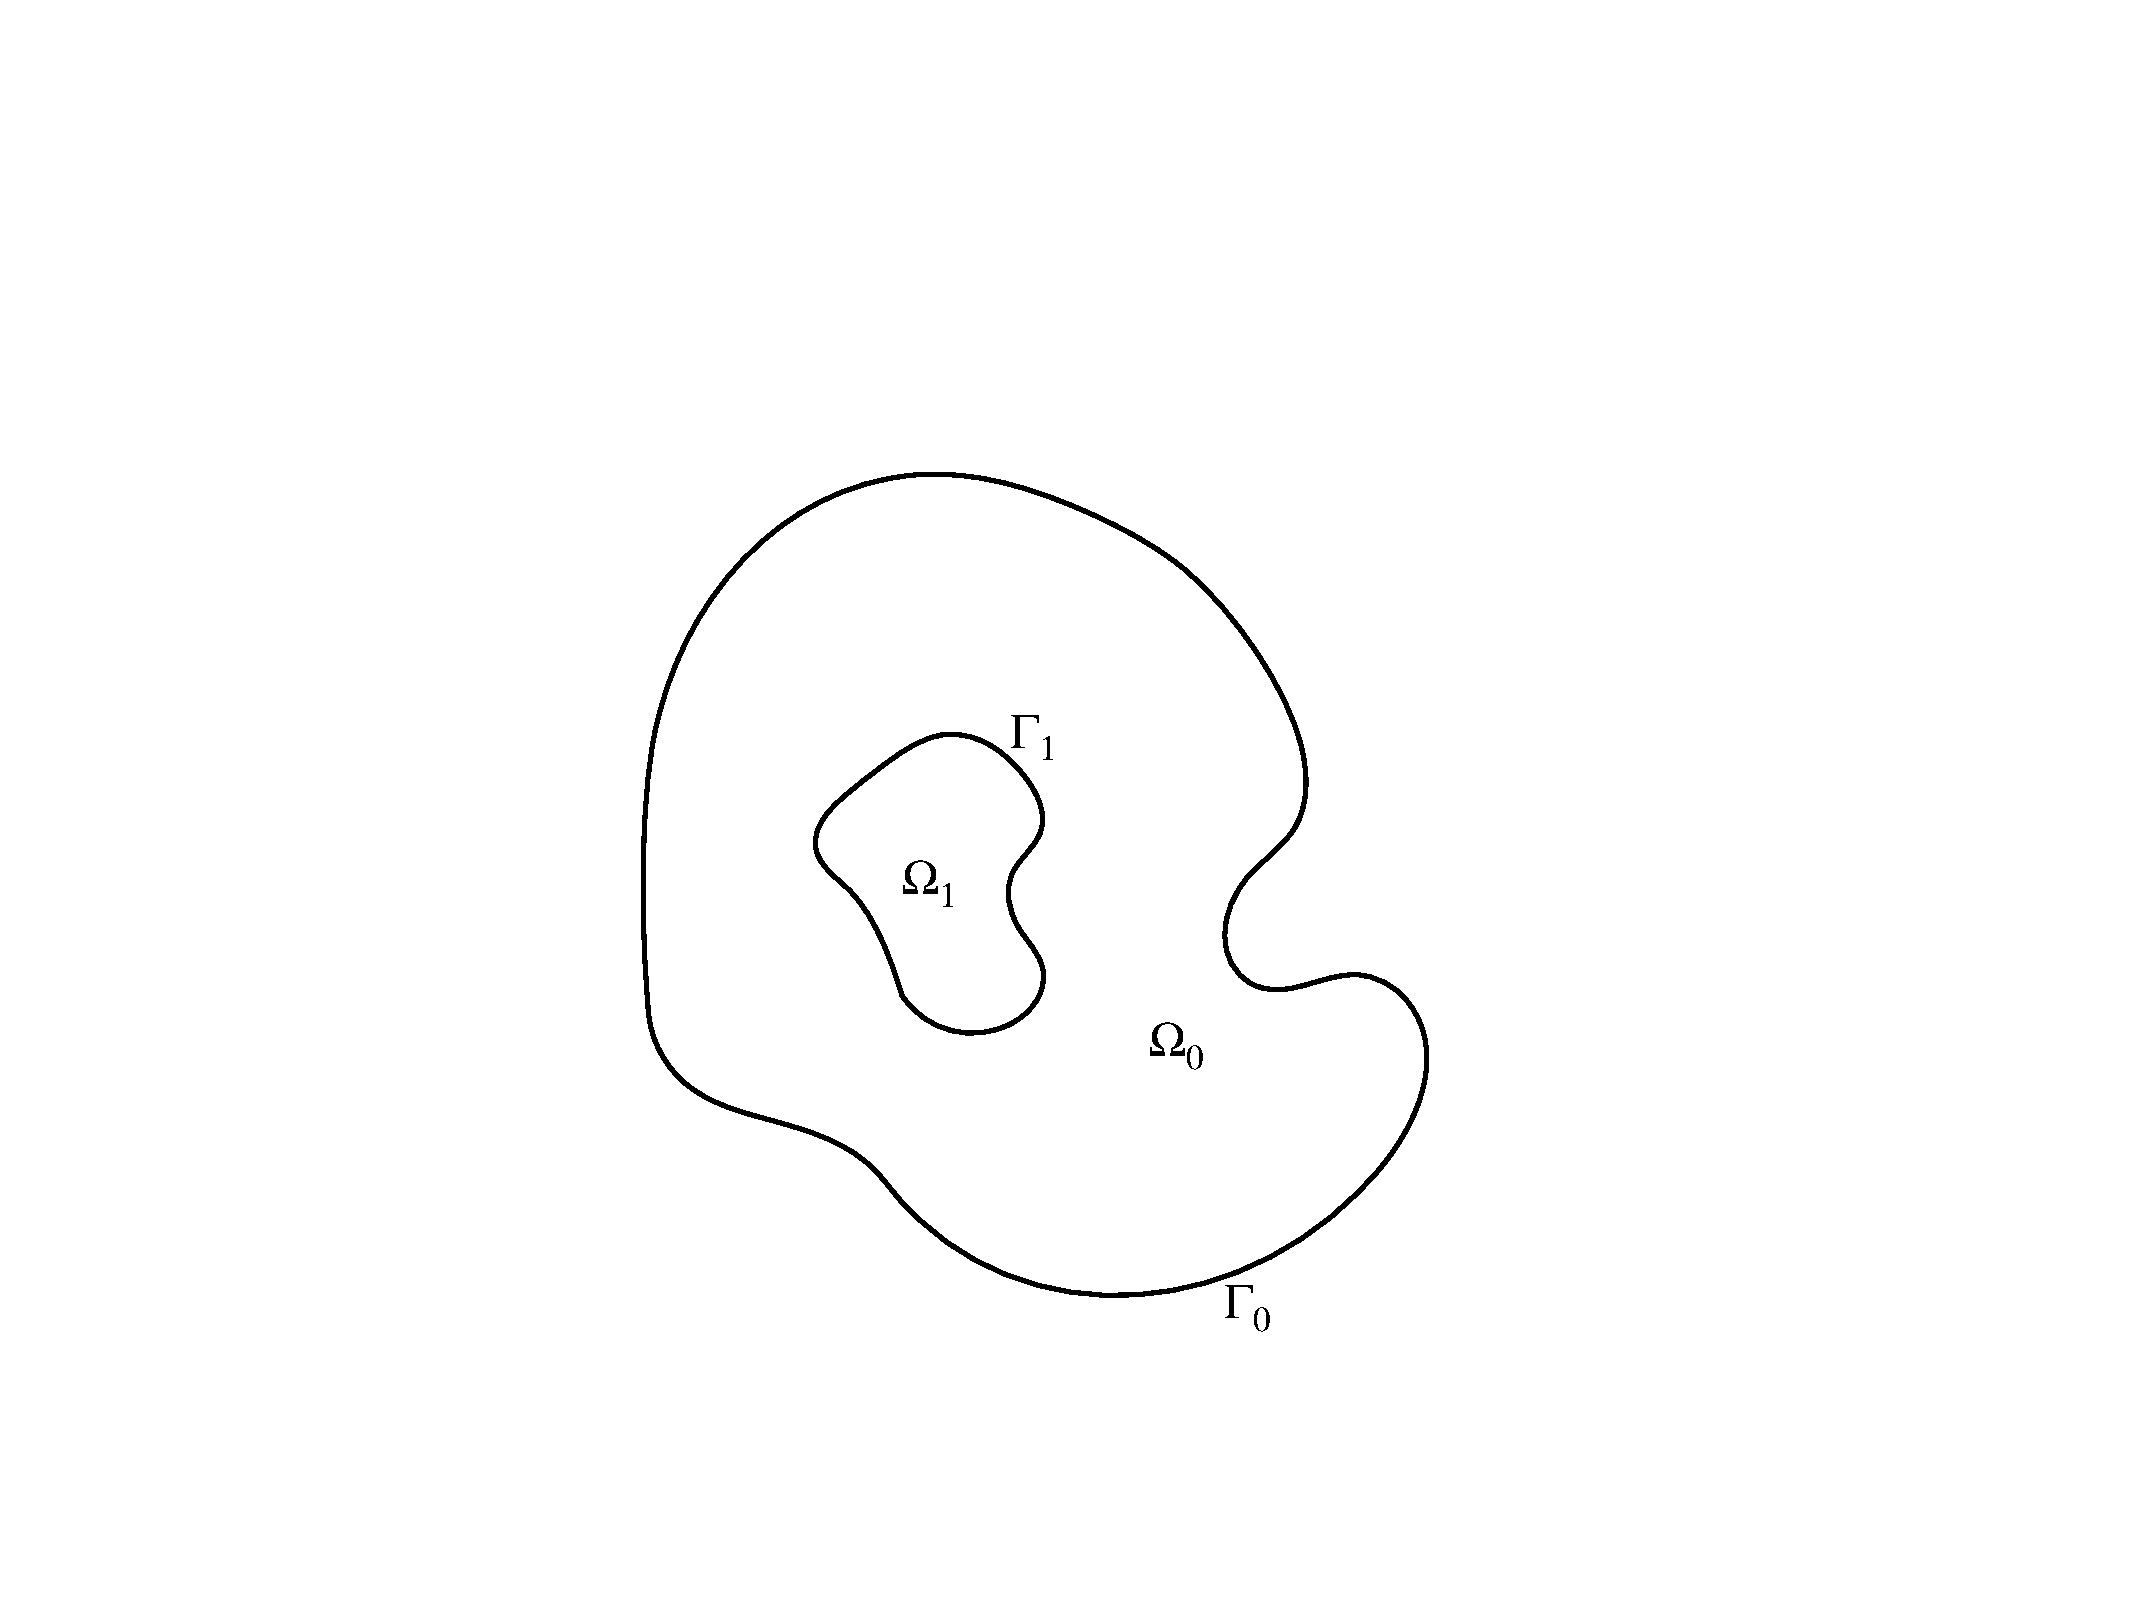
\includegraphics[width=0.3\linewidth]{media/multiply_final}
%\end{center}
%\caption{Example of a multiply connected domain with one obstacle.}
%\label{fig:1ply}
%\end{figure}

\begin{proof}
  Suppose that $k^2$ is a Neumann eigenvalue of $\Omega_{1}$.
  Let $\tilde{\bu}$ be the eigenmode corresponding to $k^2$. 
  Note that $\tilde{\bu}$ is not identically $0$ on the boundary
  of $\Omega_{1}$, which we denote by $\Gamma_1$.
  Since $\tilde{\bu}$ is an interior Neumann eigenfunction, we note that
  the surface traction corresponding to the solution, $\bt^{-}$, is $0$
  on the boundary.
  Applying \cref{thrm:rep-theorem} to the
  solution $\tilde{\bu}$ in the interior
  and taking the interior limit we get
\begin{equation}
\tilde{\bu} = \frac{1}{2}\tilde{\bu} + \cD^{\Gamma_{1}}_{k}[\tilde{\bu}] +
\cS^{\Gamma_{1}} [\bt^{-}] \implies \frac{1}{2} \tilde{\bu} - \cD^{\Gamma_{1}}_{k}[\tilde{\bu}]
= 0\, .
\end{equation}
Note that the sign of the $\bD$ operator in the
representation theorem is switched since the normal
is pointing inwards for the boundary $\Omega_{1}$.
Thus, $\tilde{\bu}$ is a non-trivial null vector of the operator 
$\frac{1}{2}\cI - \cD^{\Gamma_{1}}_{k}$. 
Furthermore since $\tilde{\bu}$ is the boundary data of 
the solution of the oscillatory Stokes equation
in $\Omega_{1}$, we get that $\cW^{\Gamma_{1}}[\tilde{\bu}] = 0$.
Setting $\bmu = \tilde{\bu}$ on $\Gamma_{1}$, and
$\bmu = 0$ on $\Gamma_{0}$, we obtain a non-trivial null
vector for the operator $\cI - 2\cD^{\Gamma}_{k} -2\cW^{\Gamma}$
on the boundary $\Gamma = \Gamma_{0} \cup \Gamma_{1}$.
\end{proof}

The spurious eigenvalues of the operator $\cI-2\cDk-2\cW$
are demonstrated in \cref{subsec:spurannulus} on an annulus,
where both the true and spurious eigenvalues can be
determined semi-analytically. 
Analogous with the observation in~\cite{zhao2015robust},
this lack of one-to-one correspondance between
the invertibility of the integral operator $\cI - 2\cD_{k} - 2\cW$
and the Dirichlet eigenvalues of the Stokes operator on multiply
connected domains also causes non-robustness and introduces near 
resonanaces for simply connected domains
which are almost multiply connected.
We demonstrate this issue numerically
in~\cref{subsec:crescent}.

\subsubsection{Dirichlet eigenvalues --- combined-field representation}
\label{subsec:mixedanalysis}

The non-robustness in using the double layer
potential representation observed above can be
remedied by using a combined-field, or mixed layer potential,
representation, i.e. setting $\bu = (\bD_{k} + i\eta \bS_{k})
\bmu$, with $\eta$ real and positive.
Imposing the Dirichlet boundary condition
and using~\cref{lem:jump-conds}, we obtain 
\begin{equation}
  (\cI - 2\cD_{k} - 2i\eta \cS_{k}) \bmu = -2 \ff \,
  \textrm{ on } \Gamma. 
\end{equation}
As with the double layer representation, this
integral equation is rank deficient for any $k$.
Instead, we consider
\begin{equation}
(\cI - 2\cD_{k} -2i\eta \cS_{k}  -2\cW)\bmu = -2 \ff \, .
\end{equation}

We now prove that for any bounded region $\Omega$
(simply or multiply connected) with $C^{2}$ boundaries,
there exists a one-to-one correspondence between the
invertibility of the operator $\cI - 2\cD_{k}
- 2i\eta \cS_{k} - 2\cW$ and the Dirichlet eigenvalues.

\begin{thrm}
  \label{thm:cfmain}
  Suppose $\Omega$ is a bounded region defined
  by the intersection of a simply connected domain $\Omega_{0}$
  and the exteriors of a finite collection bounded simply
  connected domains $\{ \Omega_{i} \}_{i=1}^{m}$. As above,
  let $\Gamma_{i}$ denote the boundary of $\Omega_{i}$ and let
  $\Gamma = \cup_{i=0}^{m} \Gamma_{i}$ denote the boundary of
  $\Omega$. Then, the operator $\cI - 2\cD_{k} - 2i\eta \cS_{k}
  - 2\cW$ is invertible if and only if $k^2$ is not a Dirichlet
  eigenvalue for the Stokes operator on $\Omega$.
\end{thrm}

\begin{proof}
  Suppose that $k^2$ is not a Dirichlet eigenvalue for the
  Stokes equation on $\Omega$. Suppose further that $\bmu$ satisfies
  \begin{equation}
    (\cI - 2\cD_{k} -2i\eta\cS_{k} - 2\cW) \bmu = 0 \, ,
    \label{eq:mlproofrep}
  \end{equation}
i.e. $\bmu$ is in the null-space
of $(\cI - 2 \cD_{k} - 2i\eta \cS_{k} - 2 \cW)$. 
Applying the operator $\cW$ to~\cref{eq:mlproofrep} and 
using~\cref{lem:propnullspacecorr}, we get
\begin{equation}
0 = \cW [(\cI - 2\cD_{k} - 2i\eta\cS_{k} - 2\cW)\bmu] = -2\cW [\bmu] \, .
\end{equation}
Thus~\cref{eq:mlproofrep} reduces to
\begin{equation}
(\cI - 2 \cD_{k} - 2i\eta \cS_{k})\bmu = 0\, .
\end{equation}
Suppose now $\bu = -2\bD_{k}[\bmu] -2i\eta\bS_{k}[\bmu]$
in $\Omega$. Then $\bu$ is a solution to the oscillatory
Stokes equation in $\Omega$, and applying~\cref{lem:jump-conds},
we get that the interior limit of the velocity
$\bu^{-} = (\cI - 2\cD_{k} -2i\eta\cS_{k}) \bmu = 0$ on $\Gamma$.
Since $k^2$ is not a Dirichlet eigenvalue for the Stokes equation
on $\Omega$, we conclude that $\bu \equiv 0$ in $\Omega$. 
This in particular implies that the interior limit of the
surface traction, denoted by $\bt^{-}$, is $0$ on $\Gamma$.
Using~\cref{lem:jump-conds} we observe that $\bt^{+}
= i\eta \bmu(\xx)$ and $\bu^{+} = \bmu(\xx)$ on $\Gamma$.
\begin{remark}
  Note that there is potential for confusion here
  in that the exterior limit with respect to $\Omega$ 
  for the boundary $\Gamma_{j}$ is the traditional interior 
  limit with respect to the obstacle region $\Omega_{j}$.
\end{remark}
We first show that $\bmu=0$ on $\Gamma_{0}$. 
To this end, note that $\bu$ is a radiating solution
of the oscillatory Stokes equation in the exterior $E$,
since $\cW[\bmu] = 0$ implies that $\int_{\Gamma} \bmu
\cdot \bnu = 0$. From the uniqueness of the impedance problem
in the exterior $E_0$ of $\Omega_0$, we conclude that
$\bu \equiv 0$ in $E_0$ as well, which in particular
implies that $\bu^{+}=0$ on $\Gamma_{0}$.   
Using the jump conditions in~\cref{lem:jump-conds}
again, we get that
$\bmu = \frac{1}{2}(\bu^{+} - \bu^{-}) = 0$ on
$\Gamma_{0}$. To show that $\bmu=0$ on
$\Gamma_{j}$, we observe that $\bu$ is also a
solution to the oscillatory Stokes equation in each
of the obstacles $\Omega_{j}$.
Applying the energy-type identity \cref{eq:greenlike}
and using the fact that 
the interior limits with respect to $\Omega_{j}$
of the surface traction and the velocity
are $i\eta \bmu$ and $\bmu$ respectively, we get
\begin{equation}
\int_{\Omega_{j}} (|e(\bu)|^{2} - \overline{k}^{2} |\bu|^2) dV 
= \int_{\Gamma_{j}} \bu \cdot \overline{\bt} dS = 
i\overline{\eta}\int_{\Gamma_{j}} |\bmu|^2 dS \, .
\end{equation}
Taking the imaginary part of the above equation,
we get
\begin{equation}
2 \text{Re}(k) \text{Im}(k) \int_{\Omega_{j}} |\bu|^2 + \text{Re}(\eta)
\int_{\Gamma_{j}} |\bmu|^2 dS = 0 \, .
\end{equation}
Since $\text{Re}(\eta)>0$, this implies that
$\bmu=0$ for $\xx \in \Gamma_{j}$, $j=1,2,\ldots m$. 
Thus, $\cI - 2\cD_{k} -2i\eta\cS_{k} -2\cW$ is
invertible when $k^2$ is not a Dirichlet eigenvalue
for the Stokes equation on $\Omega$.

From \cref{thrm:rep-theorem}, we have 
\begin{equation} 
  \bS [\bt](\xx) - \bD[\bu](\xx) = \begin{cases} 
    \bu(\xx) &\quad \xx \in \Omega \, , \\
    0 &\quad \xx \in \Omega^{C} \; .
    \end{cases}
  \end{equation}
Suppose that $k^2$ is Dirichlet eigenvalue for
the Stokes equation on $\Omega$ and let $\bu$
denote the corresponding eigenfunction and $\bt$ denote
its surface traction. Note that \cref{thrm:rep-theorem}
implies that $\cS_{k}[\bt^{-}] = 0$, since
$\bu^{-}=0$ on $\Gamma$. Applying \cref{thrm:rep-theorem}
to the pair $\bt^{-}, \bu^{-}$ and evaluating the
traction on $\Gamma$ using~\cref{lem:jump-conds},
we get
\begin{equation}
\bt^{-} = (\cDt_{k} + \frac{1}{2} \cI) \bt^{-} \, . 
\end{equation}
Combining these two identities, we get
that
\begin{equation}
(\cI - 2\cDkt -2i\eta \cS_{k}) \bt^{-} = 0 \, .
\end{equation}
As in the proof of~\cref{thm:dlmain}, letting
$c = \left< \bt^{-} ,\bnu \right>$, it follows that
\begin{equation}
  (\cI - 2\cDkt - 2i \eta \cS_{k} - 2\cW)
  (\bt^{-} - c\bnu) = 0 \, ,
\end{equation}
where $\bt^{-} - c\bnu \neq 0$.
Since $\bt^{-} - c\bnu$ is non-trivial and both
$i\eta \cS_{k}$ and $\cW$ are self-adjoint with respect
to the bilinear form \cref{eq:bi_form},
it follows from the Fredholm alternative
that the operator $\cI - 2\cDk -2i\eta \cSk - 2\cW$
is also not invertible.
\end{proof}

\subsection{Fredholm determinants}
\label{sec:dets}
Above, we established the correspondence between
the non-invertibility of certain integral equations
and Stokes eigenvalues. In this section, we show
how the Fredholm determinant can be used
as a computational tool for detecting the
non-invertibility of $\cI - 2\cD_{k} - 2\cW$.
The arguments here follow the structure of the
analogous arguments in~\cite{zhao2015robust}
for Laplace eigenvalues.

Let $\cJ_{1}(X)$ denote the space of trace class operators 
on $X$, where $X$ is a Hilbert space, which is a
subspace of the space of compact operators on $X$.
A compact operator $\cA$ with eigenvalues
$\lambda_{i}, i\in \mathbb{N}$ is in $\cJ_{1}(X)$ if
$\sum_{i} |\lambda_{i}| < \infty$.
If $\cA$, is a trace class operator, then  
the Fredholm determinant of the operator $\cI + \cA$
is defined by
\begin{equation}
\text{det}(\cI +\cA) = \prod_{i=1}^{\infty} (1+\lambda_{i}) \, .
\end{equation}
%It follows from standard results in complex
%analysis, that the Fredholm determinant is finite and well-defined if 
%$\text{det}(\cI+A) < \infty$ if $\sum_{i} |\lambda_{i}| < \infty$,
%i.e. if $A$ is in trace class.

The operator $-2\cD_{k} - 2\cW$ is trace class:
\begin{lemma}
  Suppose that $\Gamma$ is a $C^2$ curve.
  Then, $-2\cD_{k} - 2\cW \in \cJ_1(L_2(\Gamma)\otimes L_2(\Gamma))$
  for all $k$ 
\end{lemma}
\begin{proof}
Using Bessel function asymptotics, we note that the
kernel of $\cD_{k}$ given by $\TT_{\cdot,\cdot,\ell}\nu_{\ell}(\bx,\by)$
has a leading order singularity of
$|\bx-\by|^2 \log{|\bx-\by|^2}$ as $\bx\to \by$.
It follows from the criteria listed
in~\cite[Sec. 2]{bornemann2010numerical} that $\cD_{k}$
is a trace-class operator for all $k$.
Since $\cW$ is a rank-one perturbation independent of $k$,
and trace-class operators are a vector space, we conclude
that $-2\cD_{k} - 2\cW$ is also a trace-class operator for
all $k$.
\end{proof}

Let $f(k) = \text{det}(\cI - 2\cD_{k} - 2\cW)$.
First, note that $f(k)$ is an analytic function of $k$
for $k \in \mathbb{C} \setminus 0$, since the kernel
of $\cD_{k}$ is an analytic function of $k$ on that domain, 
and the Fredholm determinant is an analytic operator.

The zeros of the Fredholm determinant indicate when the
operator is not invertible. 
This is summarized as 
\begin{lem} \label{lem:detzeros}
  With $f(k)$ defined as above, $f(k) = 0$ if and only if
  $\cI - 2\cD_{k} -2\cW$ is not invertible.
\end{lem}
\begin{proof}
  The proof is standard; see, for example,
  \cite[p. 34]{simon2005trace}.
\end{proof}

When $\Omega$ is simply connected, \cref{lem:detzeros} and 
\cref{thm:dlmain} together imply that $f(k) = 0$
if and only if $k^2$ 
is a Dirichlet eigenvalue of the Stokes equation.
This reduces the problem of finding eigenvalues to
finding the roots of an analytic function.

We now show how this fact can be used to numerically
estimate the Dirichlet eigenvalues.
Suppose that $M_{k}^{N}$ is a Nystr\"{o}m discretization 
of the operator $-2\cD_{k} - 2\cW$ when the boundary 
$\Gamma$ is discretized with $N$ points. 
Let $f^{N}(k) = \text{det}(I + M_{k}^{N})$
where here $\text{det}$ is the standard matrix determinant.
Note that the discretized matrix also depends on the choice
of quadrature rule used in the Nystr\"{o}m discretization
of the operator.

In~\cite{zhao2015robust}, the authors prove that
for computing the Laplace eigenvalues on regions with 
analytic boundaries, when the integral operators are
discretized using Kress quadrature, see~\cite{kress1991boundary},
the determinant of the Nystr\"{o}m discretized operators
at the true eigenvalues converge to $0$ exponentially
in $N$.
Thus, if the eigenvalues have multiplicity $1$,
i.e. the derivative of the determinant is non-zero
at the true-eigenvalues, then the analyticity of the
discretized determinant implies that the zeros
of the determinant of the Nystr\"{o}m discretization
of the linear operator converge exponentially to
the true Dirichlet eigenvalues for Laplace's equation.

The proof presented in~\cite{zhao2015robust} carries
forward for computing the Dirichlet eigenvalues of
Stokes equation as well.
We summarize the result as
\begin{thrm}
\label{thm:mainconvfreddet}
Suppose that $\Omega$ is a simply connected
domain with an analytic boundary. Let $k_{j}^2$, $j=1,2,\ldots M$
denote all the Dirichlet eigenvalues of Stokes equation
on $\Omega$ contained in the interval $[a,b]$. 
Suppose further that all the eigenvalues have multiplicity $1$.
Let $f^{N}(k) = \text{det}(I+M^{N}_{k})$, where $M^{N}_{k}$ 
is the Nystr\"{o}m discretzation of $-2\cD_{k} - 2\cW$ with Kress
quadrature.
Then $f^{N}(k)$ has exactly $M$ zeros on the interval $[a,b]$
\note{Manas: for sufficiently large $N$?}. 
Let $\omega_{j}$, $j=1,2\ldots M$ denote the zeros of $f^{N}$.
Furthermore, there exist constants $a>0$ and $C$, 
such that $\sup_{j=1}^{M} |\omega_{j} - k_{j}| < C e^{-aN}$.
\end{thrm}

\begin{proof}
  The proof follows from small modificiations of the
  proofs contained in~\cite{zhao2015robust}. 
\end{proof}

\begin{remark}
In practice, using Kress-quadrature for large
problems is problematic owing to the global
nature of the quadrature rule.
%
\note{Manas: I do not understand the $O(N)$ cost per matrix entry
  described here in the fast-direct case ... does it somehow
  screw up compression?}
Coupling with fast direct solvers for computing determinants also results in $O(N^2 \log{N})$ 
determinant evaluation since evaluating each matrix entry costs $O(N)$, where 
$N$ is the number of discretization points on the boundary.
Over the last two decades, many high-order quadrature methods which are compatible with
fast algorithms like the fast multipole method (and fast direct solvers as well, 
since each matrix entry requires O(1) work) have been developed for solving
integral equations.
Extensive numerical evidence suggests that the zeros of the 
determinants of linear systems discretized using 
these quadrature methods are also high order approximations of Dirichlet eigenvalues
for the Stokes PDE--- the error is observed to be proportional to the quadrature error
for the eigenfunction $\bt^{-}$ associated with the eigenvalue.
We leave a proof of this to future work.
\end{remark}

\begin{remark}
The same analysis does not carry through for the operator
$\cI - 2 \cD_{k} - 2i\eta \cS_{k} - 2\cW$, 
since $\cS_{k}$ is not a trace class operator.
For brevity, let $\cM_{k} = -2\cD_{k} - 2i\eta \cS_{k} - 2\cW$.
The operator $\cM_{k}$ is 
in $\cJ_{2}(\bL^{2}(\Gamma))$ where
$\cJ_{2}(\bL^{2}(\Gamma))$ is the space of Hilbert-Schmidt operators
on $\bL^{2}(\Gamma)$ (the singular values of the operator are square
summable, as opposed to being summable).
Thus the Fredholm determinant of $\cI + \cM_{k}$
is not necessarily finite. 
However, as noted in~\cite{zhao2015robust}, the convergence
result~\cref{thm:mainconvfreddet}
should be true up to a logarithmic factor in the rate
of convergence, since the singular values of the operator
$\cM_{k}$ decay like $\frac{1}{n}$, and the
Fredholm determinant divergers logarithmically. 
In~\cref{subsec:convannulus}, we demonstrate this fact
numerically on the annulus, where the eigenvalues are
analytically known. 
\end{remark}
